	\section{آزمایشات و نتایج}
	سه مسئله نمونه طرح شده در تعریف پروژه به شرح گفته شده فرموله‌بندی شدند که جزئیات فرموله‌بندی آن‌ها در فایل
	\texttt{Main.java}
	قابل مشاهده است. با به راه‌اندازی هر جستجوگر مورد نظر در صورت پروژه در مورد هر مسئله نتایجی به دست آمد که در ادامه شرح داده می‌شوند.
	\subsection{مسئله اول: مسیریابی شهرهای رومانی}
	\begin{figure}[H]
		\centering
		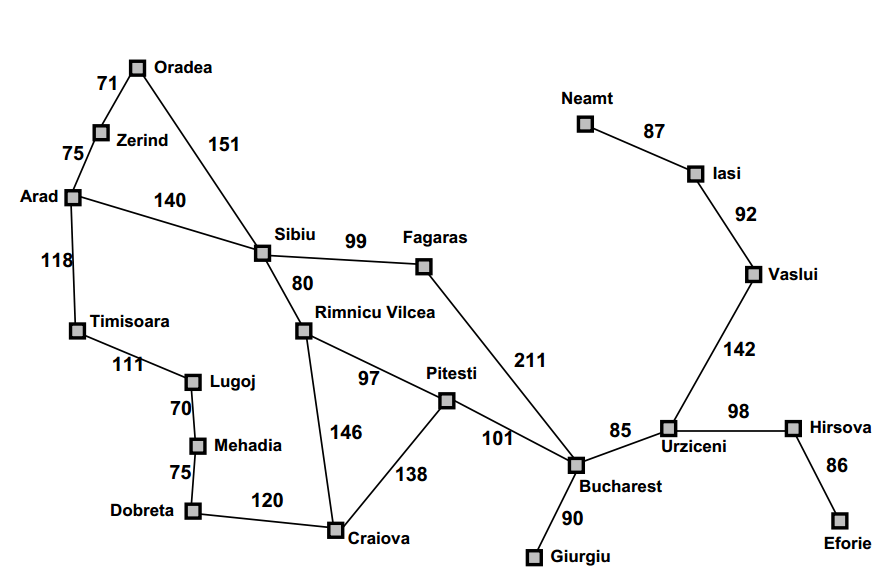
\includegraphics[width=14cm]{./Resources/p1.png}
		\caption{نقشه شهرهای رومانی}
	\end{figure}
	جزئیات فرموله‌کردن و مفروضات مورد استفاده در فرموله کردن این مسئله در بخش پیوست
	\ref{p1-app}
	قابل مشاهده است.\\
	\subsubsection{جستجوی سطح اول}
	آزمایش جستجوی سطح اول روی این مسئله با فرموله‌بندی موجود در پیوست
	\ref{p1-app}
	انجام شد و نتایج این آزمایش در جدول
	\ref{p1-bfs}
	قابل مشاهده است.
	\begin{table}[H]
		\centering
		\caption{نتایج جستجوی گراف شهرهای رومانی با استفاده از الگوریتم اول سطح.}
		\label{p1-bfs}
		\begin{tabular}{c|c}
			معیار                                   & نتیجه به دست آمده طی اجرای اگوریتم \\ \hline
			بهترین مسیر یافته شده &  \lr{Arad, Sibiu, Fagaras, Bucharest, Urziceni, Vaslui}\\
			هزینه مسیر یافته شده   &  ۶۷۷ واحد \\
			تعداد گره‌های بسط داده شده در حین جستجو & ۸۴ \\
			تعداد گره‌های مشاهده شده در حین جستجو   & ۳۳ \\
			حداکثر حافظه استفاده شده در حین جستجو   &  ۴۵                                 
		\end{tabular}
	\end{table}
	\subsubsection{جستجوی عمق اول با عمق محدود ۸}
	در پیاده‌سازی جستجوگر عمق اول در این فریم‌ورک، می‌بایست قبل از شروع جستجو مشخص شود که آیا جستجوی مورد نظر دارای عمق محدود است یا خیر. با ست کردن عمق ۸ برای این جستجوگر، نتایج آزمایش در جدول
	\ref{p1-dfs8}
	قابل مشاهده است.
	\begin{table}[H]
		\centering
		\caption{نتایج جستجوی گراف شهرهای رومانی با استفاده از الگوریتم اول عمق با عمق محدود ۸.}
		\label{p1-dfs8}
		\begin{tabular}{c|c}
			معیار                                   & نتیجه به دست آمده طی اجرای اگوریتم \\ \hline
			بهترین مسیر یافته شده &  \lr{Arad, Zerind, Oradea, Sibiu, Fagaras, Bucharest, Urziceni, Vaslui}\\
			هزینه مسیر یافته شده   &  ۸۳۴ واحد \\
			تعداد گره‌های بسط داده شده در حین جستجو & ۲۲ \\
			تعداد گره‌های مشاهده شده در حین جستجو   & ۱۴ \\
			حداکثر حافظه استفاده شده در حین جستجو   &  ۱۴                                 
		\end{tabular}
	\end{table}
	
	\subsubsection{جستجوی A*}
	در این جستجو، تابع شهودی مورد استفاده، فاصله واقعی هر شهر تا شهر مقصد بوده که از وب نتایج یافت شدند. جزئیات این تابع در پیوست
	\ref{p1-app}
	قابل مشاهده است. نتایج این آزمایش نیز در جدول
	\ref{p1-astar}
	ذکر شده است.
		\begin{table}[H]
		\centering
		\caption{نتایج جستجوی گراف شهرهای رومانی با استفاده از الگوریتم اول عمق با عمق محدود ۸.}
		\label{p1-astar}
		\begin{tabular}{c|c}
			معیار                                   & نتیجه به دست آمده طی اجرای اگوریتم \\ \hline
			بهترین مسیر یافته شده &  \lr{Arad, Sibiu, Fagaras, Bucharest, Urziceni, Vaslui}\\
			هزینه مسیر یافته شده   &  ۶۷۷ واحد \\
			تعداد گره‌های بسط داده شده در حین جستجو & ۳۲ \\
			تعداد گره‌های مشاهده شده در حین جستجو   & ۱۲ \\
			حداکثر حافظه استفاده شده در حین جستجو   &  ۲۴                                 
		\end{tabular}
	\end{table}
	\subsection{مسئله دوم: پازل ۸تایی}
	\subsubsection{جستجوی اول عمق گرافی}
	در جستجوی اول عمق گرافی نمونه داده شده در تعریف پروژه به مشکل عدم وجود حافظه کافی برخورد کردیم که با تغییر نمونه ورودی به ورودی زیر (فقط به عنوان تست) می‌توان پاسخ مناسب از آن گرفت:
	$1, 0, 2, 3, 4, 5, 6, 7, 8$
	\subsubsection{جستجوی دو جهته}
	با اجرای این الگوریتم با حالت اولیه ذکر شده در تعریف پروژه، که زمان بسیار زیادی برای اجرا نیاز داشت، به نتیجه‌ای نرسیدیم. اما با دادن حالت
	$ 1, 4, 2, 0, 3, 5, 6, 7, 8$
	به عنوان حالت اولیه، به نتایج ذکر شده در جدول
	\ref{p2-bds}
		رسیدیم.
		\begin{table}[H]
		\centering
		\caption{نتایج جستجوی دو جهته فضای حالت پازل ۸ تایی.}
		\label{p2-bds}
		\begin{tabular}{c|c}
			معیار                                   & نتیجه به دست آمده طی اجرای اگوریتم \\ \hline
			بهترین مسیر یافته شده &  \lr{012345678, 102345678, 142305678, 142035678}\\
			هزینه مسیر یافته شده   & ۳ \\
			تعداد گره‌های بسط داده شده در حین جستجو & ۹ \\
			تعداد گره‌های مشاهده شده در حین جستجو   & ۵ \\
			حداکثر حافظه استفاده شده در حین جستجو   & ۱۱                                 
		\end{tabular}
	\end{table}
	\subsubsection{جستجوی A* با تابع شهودی فاصله مستقیم}
	با اجرای الگوریتم داده شده و تابع شهودی مورد نظر، با حالت اولیه ذکر شده در قسمت قبل، در تعریف پروژه به نتایج ذکر شده در جدول
	\ref{p2-astar}
	رسیدیم.
		\begin{table}[H]
			\centering
			\caption{نتایج جستجوی دو جهته فضای حالت پازل ۸ تایی.}
			\label{p2-astar}
			\begin{tabular}{c|c}
				معیار                                   & نتیجه به دست آمده طی اجرای اگوریتم \\ \hline
				بهترین مسیر یافته شده &  \lr{012345678, 102345678, 142305678, 142035678}\\
				هزینه مسیر یافته شده   & ۳ \\
				تعداد گره‌های بسط داده شده در حین جستجو & ۱۲ \\
				تعداد گره‌های مشاهده شده در حین جستجو   & ۵ \\
				حداکثر حافظه استفاده شده در حین جستجو   & ۱۲                                 
			\end{tabular}
		\end{table}
	\subsection{مسئله سوم: مبلغین مذهبی و آدم‌خوارها}
	با پیاده‌‌سازی و فرموله‌بندی این سوال در متد
	\texttt{p3}
	فایل
	\texttt{Main.java}
	به اجرای الگوریتم‌های جستجوی مختلف روی این سوال پرداخته شد.
	\subsubsection{جستجوی سطح اول}
	نتایج جستجوی سطح اول در جدول
	\ref{p3-bfs}
	ذکر شده است.
			\begin{table}[H]
			\centering
			\caption{نتایج جستجوی سطح اول مسئله مبلغیم مذهبی و آدم‌خوارها}
			\label{p3-bfs}
			\begin{tabular}{c|c}
				معیار                                   & نتیجه به دست آمده طی اجرای اگوریتم \\ \hline
				بهترین مسیر یافته شده & (در سمت اولیه رود) ۳ آدم‌خوار و ۳ مبلغ، ۱ آدم‌خوار و ۳ مبلغ، ۱ آدم‌خوار و ۱ مبلغ، ۰ آدم‌خوار و ۰ مبلغ\\
				هزینه مسیر یافته شده   & ۳ \\
				تعداد گره‌های بسط داده شده در حین جستجو & ۳۲ \\
				تعداد گره‌های مشاهده شده در حین جستجو   & ۲۰ \\
				حداکثر حافظه استفاده شده در حین جستجو   & ۳۳                                 
			\end{tabular}
		\end{table}	 
	\subsubsection{جستجوی عمق اول با افزایش تدریجی عمق}
	نتایج جستجوی عمق اول با افزایش تدریجی عمق در جدول
	\ref{p3-dfs}
	قابل مشاهده است.
	\begin{table}[H]
		\centering
		\caption{نتایج جستجوی سطح اول مسئله مبلغیم مذهبی و آدم‌خوارها}
		\label{p3-dfs}
		\begin{tabular}{c|c}
			معیار                                   & نتیجه به دست آمده طی اجرای اگوریتم \\ \hline
			بهترین مسیر یافته شده & (در سمت اولیه رود) ۳ آدم‌خوار و ۳ مبلغ، ۱ آدم‌خوار و ۳ مبلغ، ۱ آدم‌خوار و ۱ مبلغ، ۰ آدم‌خوار و ۰ مبلغ\\
			هزینه مسیر یافته شده   & ۳ \\
			تعداد گره‌های بسط داده شده در حین جستجو & ۵۸ \\
			تعداد گره‌های مشاهده شده در حین جستجو   & ۶۱ \\
			حداکثر حافظه استفاده شده در حین جستجو   & ۲۸                                 
		\end{tabular}
	\end{table}	 
	
	
